\documentclass{beamer}

\usepackage{gensymb}
\usepackage[utf8]{inputenc}
\DeclareUnicodeCharacter{00A0}{ }%Permet d'éviter certains conflits de caractères invisibles
\usepackage{amssymb}            % Principaux symboles
%\usepackage{fontspec}
%\usepackage{xunicode}
%\usepackage{xltxtra}
\usepackage[frenchb]{babel}
%\defaultfontfeatures{Scale=MatchLowercase}
%\setmainfont[Mapping=tex-text,Ligatures={Common, Historical}]{Linux Libertine O}
%\setsansfont[Mapping=tex-text]{Linux Biolinum O}
%\setmonofont[Scale=0.75]{DejaVu Sans Mono}

%% Packages pour le texte
%\usepackage[misc,geometry]{ifsym}	% Police numéros battons
\usepackage{pifont}		% Police \ding
\usepackage{eurosym}		% Symbole de l'euro
\usepackage{soul}		% Souligner
\usepackage{enumerate}		% Listes
\usepackage{verbatim}		% Codes source
\usepackage{moreverb}		%	et listings
\usepackage{textcomp}
\usepackage{multicol}

%% Packages pour les tableaux
\usepackage{array}		% Outils supplémentaires
\usepackage{multirow}		% Colonnes multiples
\usepackage{tabularx}		% Largeur totale donnée
\usepackage{longtable}		% Sur plusieurs pages

%% Les packages pour les dessins
\usepackage{graphicx}		% Insertion de figures
%\usepackage{picins}		% Dans un paragraphe
\usepackage{epic}		% Capacités graphiques
\usepackage{eepic}		% 	étendues
\usepackage{afterpage}		% Voir page 69
\usepackage{rotating}		% Tourner du texte
\usepackage{caption}		% Légendes
% \addto\captionsfrench{\def\figurename{}}

%% Packages pour les maths
\usepackage{amsmath}		% Commandes essentielles
\usepackage{amssymb}		% Principaux symboles
\usepackage{mathrsfs}		% Police calligraphique
\usepackage{theorem}		% Théorèmes
%\usepackage{tikz}		% Courbes
\usepackage{esvect}            % Vecteurs
%\usetikzlibrary{shapes,arrows,shadows}
\usepackage{pgf}
%\usetikzlibrary{arrows}
% Packages pour la physique
%\usepackage{sistyle}		% Unités
\usepackage[version=3]{mhchem}	% Formules chimiques
\usepackage{etex}
%\usepackage{m-pictex,m-ch-en}

%\usepackage{media9}
\usepackage{multimedia}		% Vidéos dans la présentation
%\usepackage{movie15}

%Ajout d'images de fond:
\usepackage{eso-pic}
\usepackage{wallpaper}

\usepackage{ccicons}		% Licence creativecommons

%\SIdecimalsign{,}


\AtBeginSection[]
{
  \begin{frame}
    \frametitle{Sommaire}
    \begin{multicols}{2}
      {\small
				\setcounter{tocdepth}{2}
        \tableofcontents[currentsection, hideothersubsections]}
    \end{multicols}
  \end{frame}
}

\usetheme{Warsaw}

\usepackage{listings}
\usepackage[babel=true]{csquotes}
\lstset{language=Python, tabsize=2, breaklines=true, showstringspaces=false}

\useoutertheme{infolines}
\setbeamersize{text margin left=1cm,text margin right=1cm}

\title{La folie des grandeurs}
\subtitle{Le monde est fou}
\author{Tristan, Alexis, Thomas, Thibaut}

\begin{document}

\begin{frame}
  \titlepage
\end{frame}

\begin{frame}
    \frametitle{Sommaire}
    \begin{multicols}{2}
      {
		\setcounter{tocdepth}{1}
        \tableofcontents
      }
    \end{multicols}
\end{frame}

\section{La folie}

\begin{frame}
  \begin{displayquote}
    Folie~: Dérèglement mental, démence : Sombrer dans la folie.

    Démence~: (latin~: demens, folie) Sérieuse perte ou réduction des capacités cognitives suffisamment importante pour retentir sur la vie d'un individu et entraîner une perte d'autonomie.
  \end{displayquote}
\end{frame}

\begin{frame}
  \begin{itemize}
    \item réaction inappropriée ou disproportionnée face à la perception de la réalité. Relatif à un individu ou un groupe d'individus~;
    \item Action sans but, homme lunatique.
  \end{itemize}
\end{frame}

\section{Le monde est fou}

\begin{frame}{Problématique}
  \begin{center}
    La folie reflète-t-elle une vision de groupe ?
  \end{center}
\end{frame}

\begin{frame}{Société}
  La folie est relative à la société ou à un groupe d'individus.
  Chaque société pense l'autre folle. Jugement relatif.

  Sortir de la norme ou de la majorité.

  Penser comme tout le monde est un risque de mal interpréter la réalité~: actions inappropriées, aliénation à la masse.
\end{frame}

\begin{frame}{Sciences alternatives}
	\begin{itemize}
	 \item le scientisme est une vision du monde, apparue au XIXe siècle~;
	 \item Énergie libre
		\begin{center}
			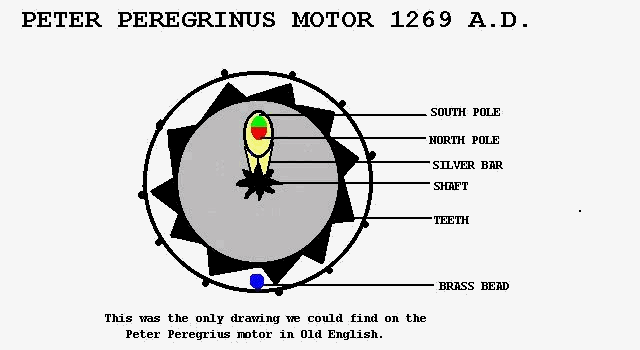
\includegraphics[width=5cm]{../Images/energie_libre.png}
		\end{center}

	\end{itemize}

\end{frame}


\begin{frame}{Sectes}
  Seul contre le monde~: raisonnement disproportionné, souvent illogique.
  \begin{center}
    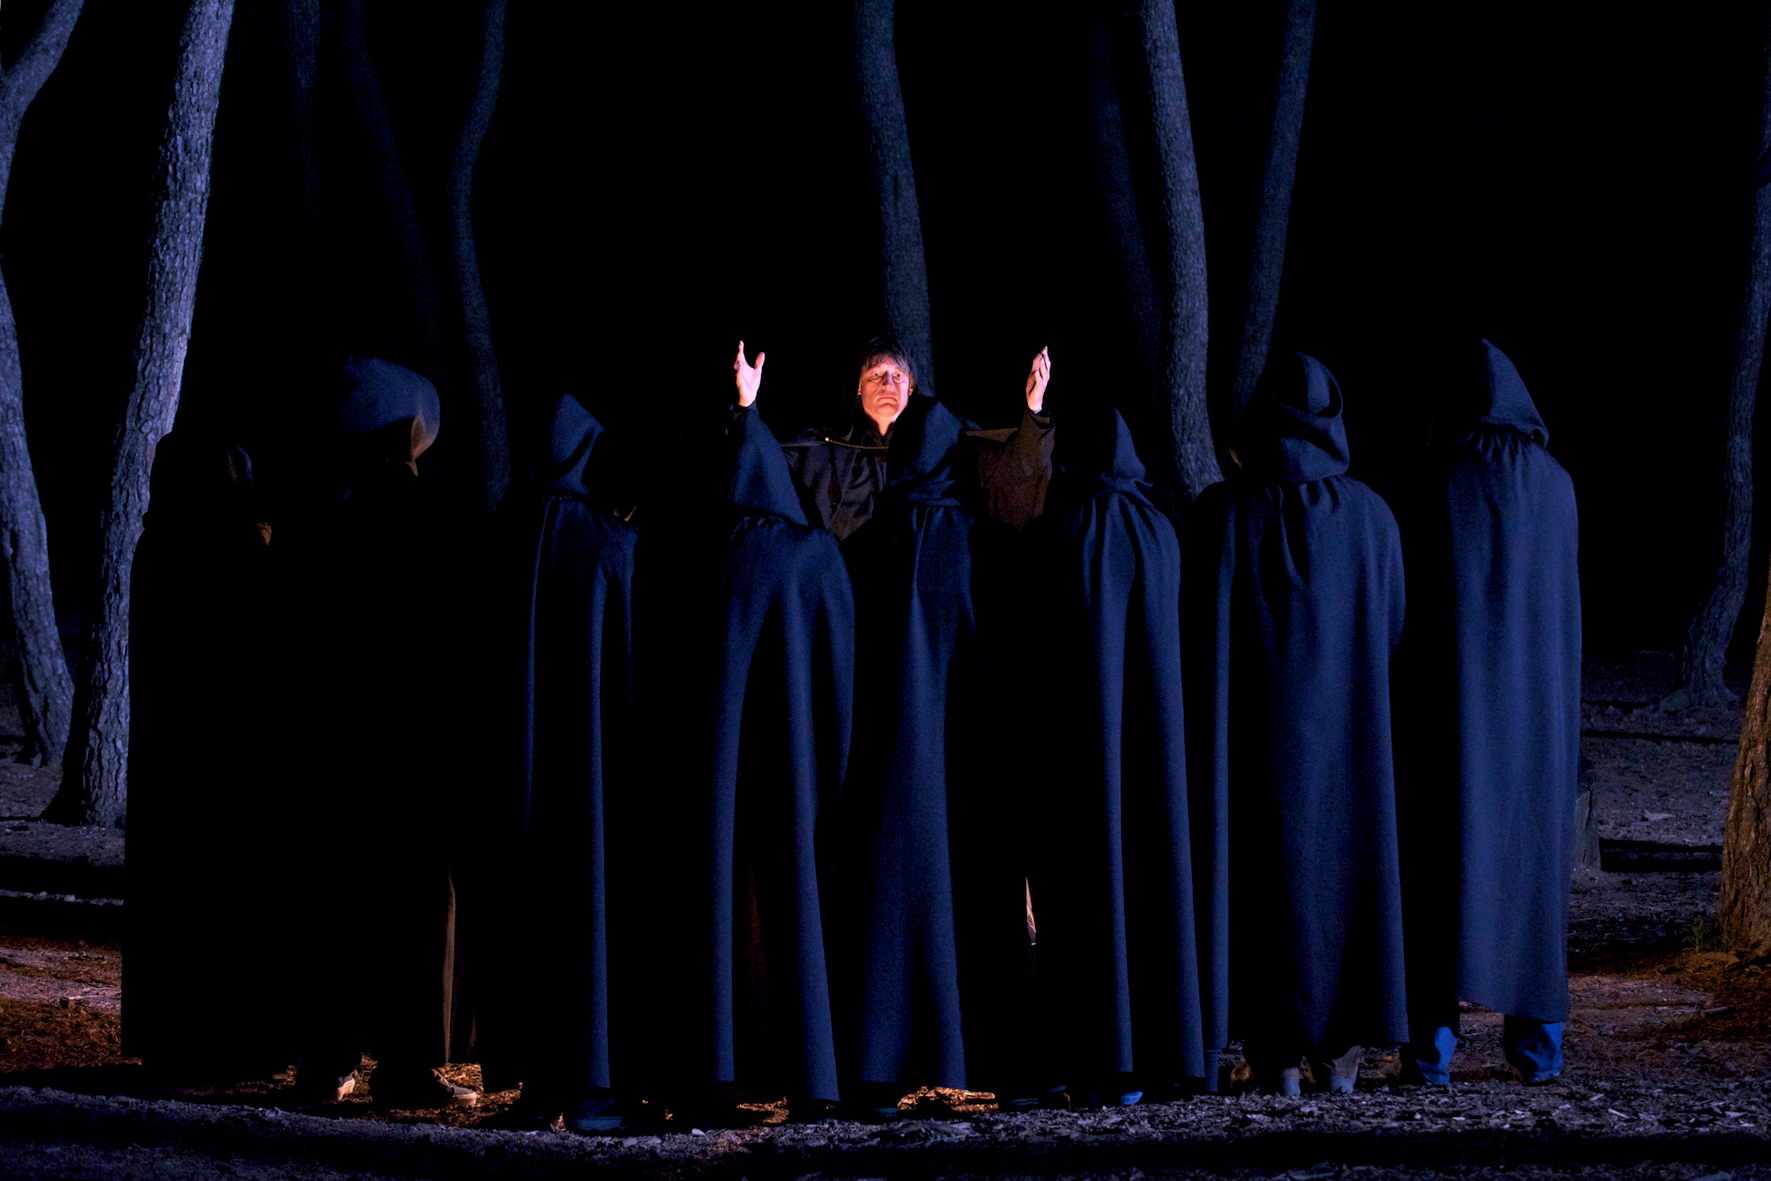
\includegraphics[width=5cm]{../Images/secte.png}
  \end{center}
\end{frame}

\begin{frame}{Le monde est condamné à être fou}
  On glorifie ce qui sort de l'ordinaire pcq notre modèle globalisé nous force à nous démarquer : c'est la folie qui nous fait évoluer.

\end{frame}

\section{Folie des grandeurs}

\begin{frame}{Problématique}
  \begin{center}
    Les désirs de l'homme sont-ils sans fin ?
  \end{center}
\end{frame}

\begin{frame}{Démesure}
  Démesure~: sortir de la mesure~; indéfini.

  Relatif aux sociétés et à leurs époques, chercher plus grand.
\end{frame}

\begin{frame}{Besoins artificiels}
  \begin{itemize}
    \item l'homme ne se contente jamais de ce qu'il possède~;
    \item but infini, flou, absurde, quête perdue d'avance~;
    \item démence~;
    \item demesure, originalité dans les besoins.
  \end{itemize}
\end{frame}

\begin{frame}{Productivisme et consumérisme}
  Sur-production et sur-consommation.
  Alimentation et gaspillage.
  \begin{center}
    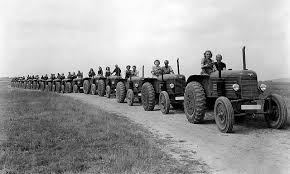
\includegraphics[width=5cm]{../Images/urss.png}
    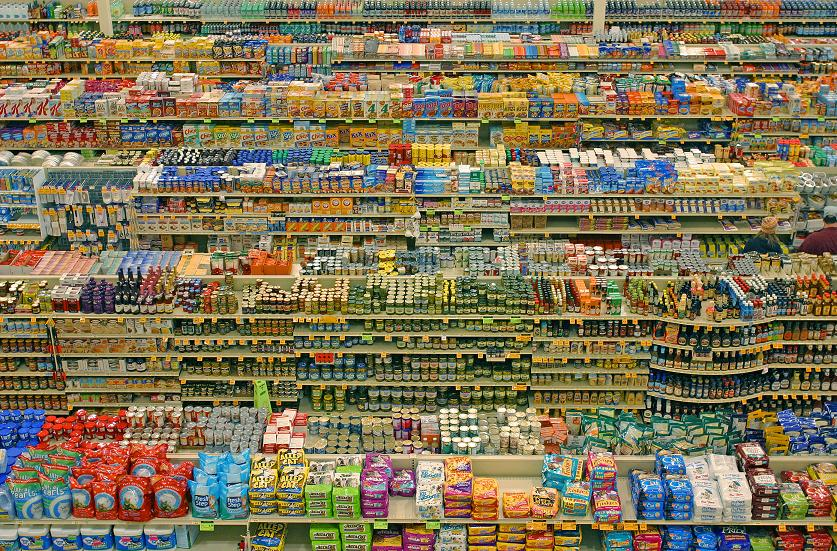
\includegraphics[width=5cm]{../Images/productivisme.jpeg}
	\end{center}
\end{frame}

\begin{frame}{Menace scientifique : exemple de l'armement}
  \begin{center}
    Nous avons la capacité de détruire plusieurs fois la planète.
    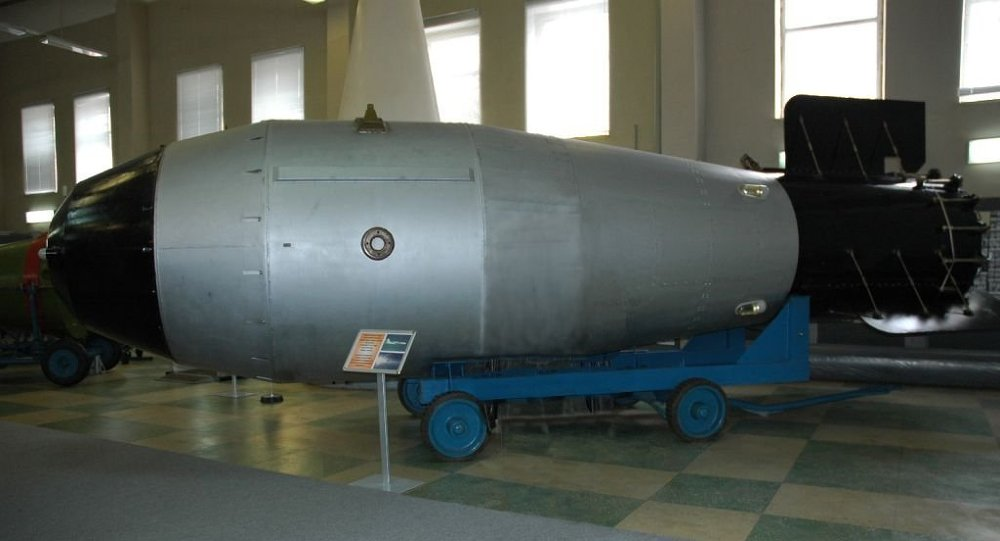
\includegraphics[width=10cm]{../Images/bombe.jpg}
  \end{center}

\end{frame}

\begin{frame}{Conclusion}
  \begin{center}
    Les désirs de l'homme semblent sans fin. \\
    $=>$ changer de paradigme ?

  \end{center}

\end{frame}

\end{document}




\section{La société}

\subsection{Une humanité qui se perd}
\begin{frame}{Une humanité qui se perd}
  Plus le temps de vivre, temps impossible à sacrifier.
  Concept d'identité, oppresseur.
\end{frame}

\subsection{Productivisme et consumérisme}



\section{Grandeur et démesure}

\subsection{Repousser les frontières au-delà de la terre}
\begin{frame}{Repousser les frontières au-delà de la terre}
  Espace
\end{frame}
